\documentclass{beamer}
\usepackage{amssymb, amsfonts, latexsym, amsthm, amsmath, framed, esvect, parskip}
\usepackage{amsmath, amssymb, framed, tcolorbox, mathrsfs, xcolor, graphicx}
\usepackage{multirow,booktabs, makecell, svg}
\usepackage{eso-pic}
\usepackage[backend=biber,style=numeric,sorting=none]{biblatex}
\setbeamerfont{footnote}{size=\tiny}
\addbibresource{ref.bib}
\tcbuselibrary{theorems}
\usepackage{listings}
\definecolor{green}{rgb}{0,0.6,0}
\definecolor{gray}{rgb}{0.5,0.5,0.5}
\definecolor{mauve}{rgb}{0.58,0,0.82}
\lstset{
    frame=none,
    language=Java,
    showstringspaces=false,
    columns=fullflexible,
    basicstyle = \ttfamily\small,
    numbers=none,
    numberstyle=\tiny\color{gray},
    keywordstyle=\color{blue},
    commentstyle=\color{green},
    stringstyle=\color{mauve},
    breaklines=true,
    morekeywords={function},
    breakatwhitespace=true,
    tabsize=4
}

% Beamer theme setting
\definecolor{myteal}{cmyk}{0.5,0,0.15,0}
\usecolortheme[named=myteal]{structure}
\definecolor{my-yellow}{cmyk}{0,0.2,0.7,0,1.00}
\definecolor{my-blue}{cmyk}{0.80, 0.13, 0.14, 0.04, 1.00}
\definecolor{my-green}{cmyk}{0.4,0,0.4,0,1.00}
\tcbset{
defstyle/.style={fonttitle=\bfseries\upshape, colback=my-yellow!5,colframe=my-yellow!80!black},
theostyle/.style={fonttitle=\bfseries\upshape, colback=my-blue!5,colframe=my-blue!80!black},
corstyle/.style={fonttitle=\bfseries\upshape, colback=my-green!5,colframe=my-green!80!black},
}
\usetheme{Madrid}
\setbeamertemplate{itemize items}[triangle]
\setbeamertemplate{enumerate items}[default]

\newcommand\AtPagemyUpperLeft[1]{\AtPageLowerLeft{%
\put(\LenToUnit{0.9\paperwidth},\LenToUnit{0.9\paperheight}){#1}}}

\title{Replicating Side Channel Attacks on RISC-V}
\author{Ben Chen, Shuwei Zhang, Jikun Liao}
\institute{Dept of Computer Science and Technology, SUSTech}
\date{\today}

\begin{document}
\frame{\titlepage}

\begin{frame}
    \frametitle{Introduction}
    In this project, we
    \begin{itemize}[<+->]
        \item spent 5 weeks to survey the microarchitectural vulnerabilities
        \item replicated Spectre, Phantom and Downfall on x86-64 CPU
        \item analyzed the attack surfaces on XiangShan
        \item set up the workflow for running XiangShan on simulator
        \item migrated the attacks on XiangShan
    \end{itemize}
\end{frame}

\begin{frame}
    \frametitle{Background}
    \framesubtitle{Side-Channel Attacks}
    Side channel attacks exploit unintended information leakage in
    \begin{itemize}[<+->]
        \item energy: voltage, power, radiation...
        \item timing: execution cost $\rightarrow$ branching result
        \item cache: timing difference $\rightarrow$ data present or not in cache
        \item contention: cross-core interrupts, bus, and other resource contention $\rightarrow$ network fingerprints
        \item other architecture: MWAIT\cite{mwait} status change encoded in user-readable register
    \end{itemize}
\end{frame}

\begin{frame}
    \frametitle{Background}
    \framesubtitle{Cache Side-Channel}
    \begin{columns}
        \begin{column}{0.5\textwidth}
            \begin{itemize}
                \item Flush+Reload: Flush all cache of attacker's probe array, encode victim's secret in offset of probe array and reload to time the difference
                \item Prime+Probe: Fill the cache with attacker's probe array, and victim's cache evict a element of probe array in cache, so attacker can tell which one is evicted
            \end{itemize}
        \end{column}
        \begin{column}{0.5\textwidth}
            \begin{figure}
                \centering
                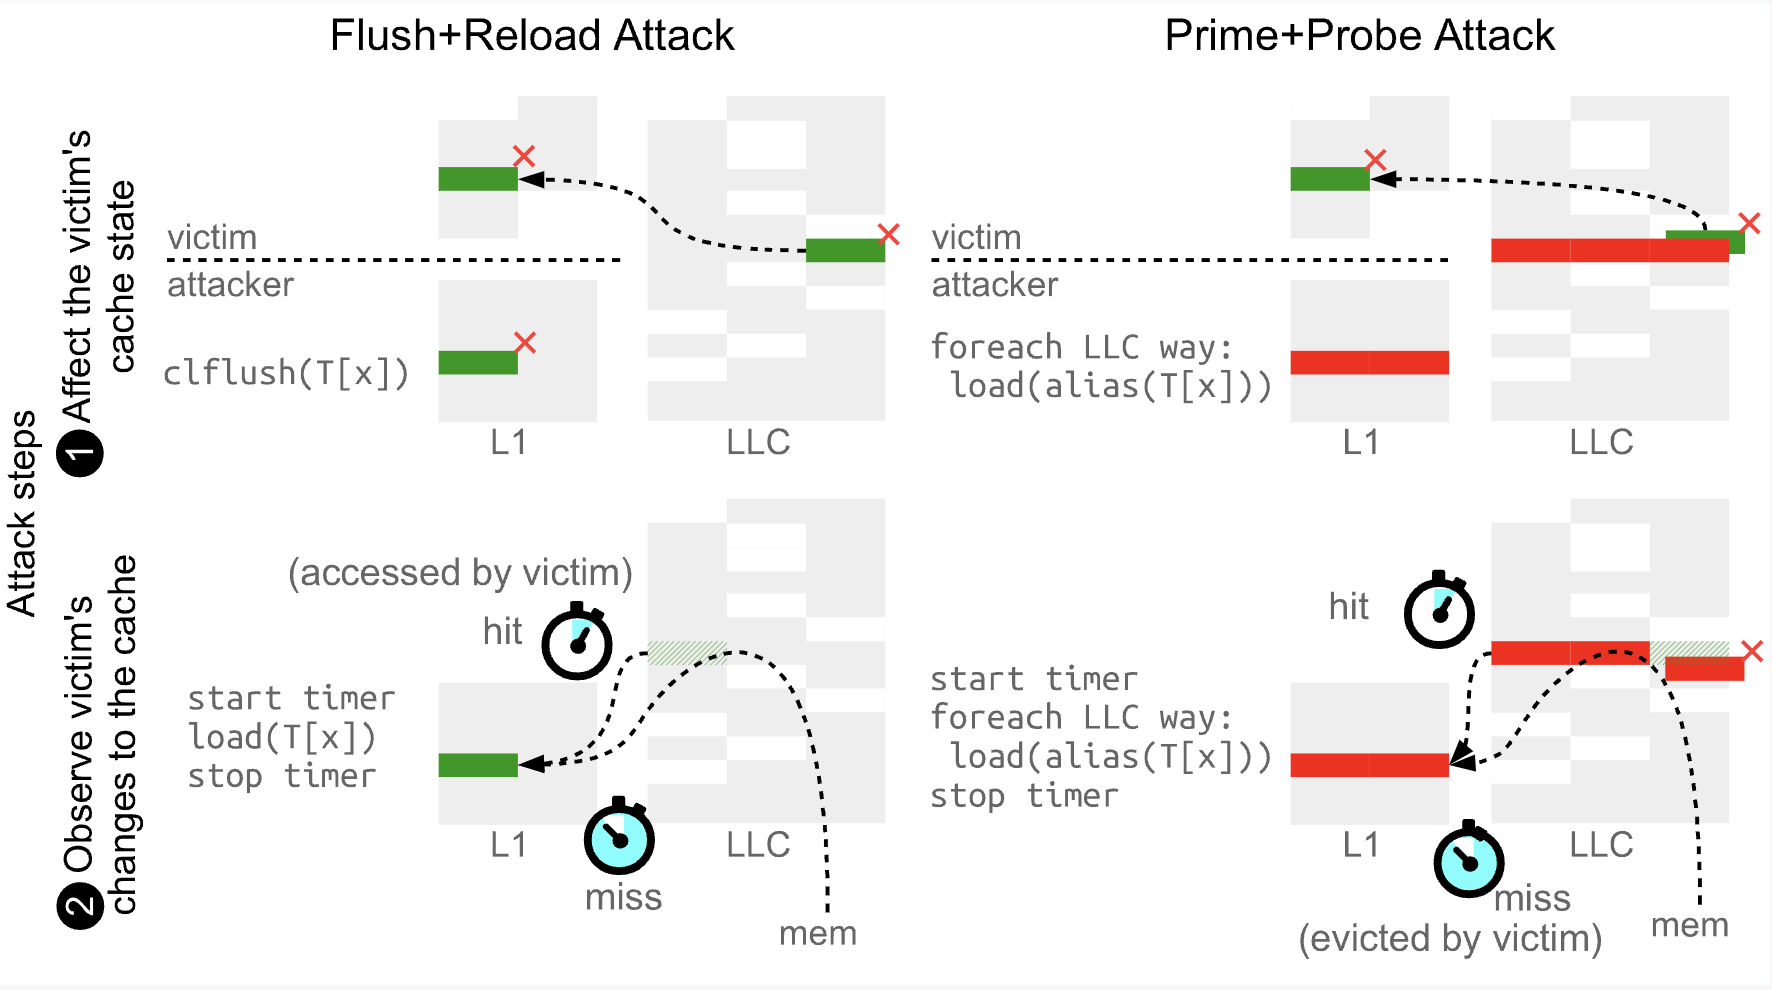
\includegraphics[width=1\linewidth]{Figure/cache-attack.png}
            \end{figure}
        \end{column}
    \end{columns}
\end{frame}

\begin{frame}
    \frametitle{Motivation}
    We've seen plentiful defense on RISC-V
    \begin{itemize}
        \item SafeSpec\cite{safespec}: Blocking unsafe loads from altering the data cache
        \item SpectreGuard\cite{spectreguard}/SpecTerminator\cite{specterminator}: Marking the unsafe load to prevent speculative load
    \end{itemize}
    but few attack on RISC-V and especially on XiangShan
    \begin{itemize}
        \item A Secure RISC\cite{a-secure-risc}: Attack I\$ on C906 \& U74
    \end{itemize}
\end{frame}

\begin{frame}{Motivation}
\AddToShipoutPictureFG*{
  \AtPagemyUpperLeft{{
\includegraphics[width=1cm,keepaspectratio]{Figure/xs-logo.png}}}
}

XiangShan is a open-source RISC-V core IP
\begin{itemize}[<+->]
    \item developed by ICT of CAS, led by Yungang Bao
    \item out of order, superscalar
    \item runs RISC-V RV64GCV, Linux-capable, FPGA-capable
    \item written in Chisel, agile development and verification
\end{itemize}
    \onslide<5>{Is XiangShan vulnerable to Spectre or so?}
\end{frame}

\begin{frame}[fragile]
    \frametitle{Spectre}
    \framesubtitle{Spectre on x86}
    Vulnerable code in victim
    \begin{lstlisting}
    uint8_t array[160] = {1, 2, ..., 16};
    char* secret = "Secret goes here!";
    
    void victim_function(size_t x) {
       if (x < array1_size) { // array1_size = 16
           temp &= array2[array1[x] * CACHELINE_SIZE];
       }
    }
    \end{lstlisting}
    
\end{frame}

\begin{frame}[fragile]
    \frametitle{Spectre}
    \framesubtitle{Spectre on x86}
    Training the branch predictor
    \begin{lstlisting}
    for (int x = 0; x < ENTRY_SIZE; ++x) {
        victim_function(x);
    }
    flush_cache(array2);
    victim_function(secret[i++]);
    
    for (int i = 0; i < 256; i++) {
        addr = &array2[i * CACHELINE_SIZE];
        time1 = __rdtscp(&junk); /* READ TIMER */
        junk = * addr; /* MEMORY ACCESS TO TIME */
        time2 = __rdtscp(&junk) - time1; 
        /* READ TIMER & COMPUTE ELAPSED TIME */
        if (time2 <= CACHE_HIT_THRESHOLD)
            results[i]++;
    }
    \end{lstlisting}
    
\end{frame}

\begin{frame}
    \frametitle{Spectre}
    \framesubtitle{Spectre on XiangShan}
    XiangShan Branch Predictor
    \begin{center}
        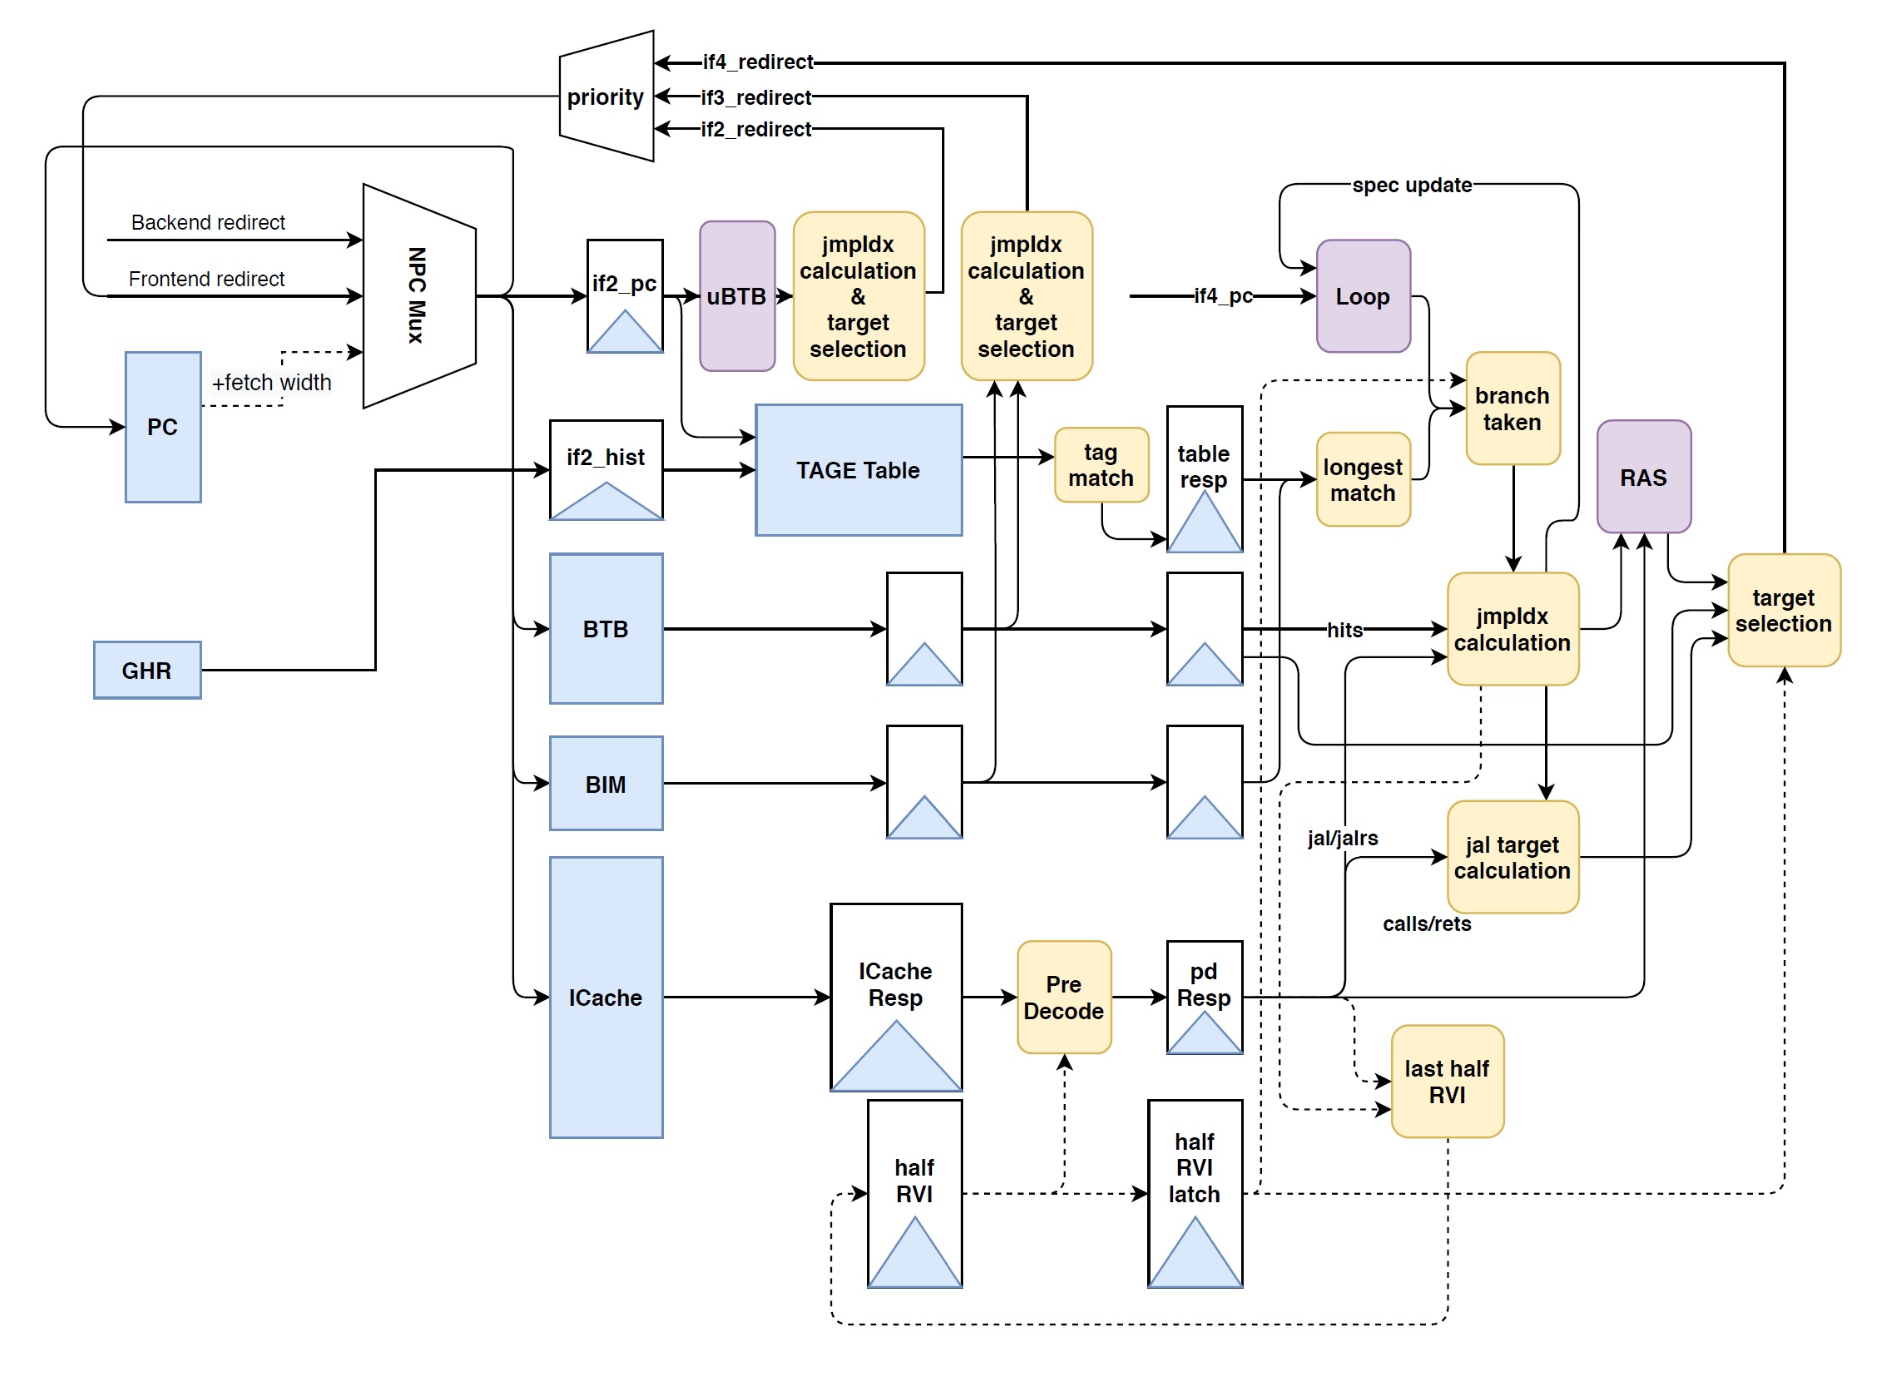
\includegraphics[width=0.7\textwidth]{Figure/xs-branch-predictor.png}
    \end{center}
\end{frame}

\begin{frame}
    \frametitle{Spectre}
    \framesubtitle{Spectre on XiangShan}
    \begin{itemize}
        \item Branch predictors: $\mu$BTB, BTB, TAGE, RAS and loop predictor\newline
        TAGE + loop predictor $\rightarrow$ disable the original attack
        \item Speculative Execution\newline
        Out-of-order, multiple issue $\rightarrow$ Spectre-vulnerable
        \item Cache: L1 \$ L2\newline
        8 ways, 256 sets, 64B each line $\rightarrow$ enough to encode a character
        \item Timer and cache manipulation\newline
        \texttt{rdcycle} cycle-level timer, \texttt{fence.i} memory barrier
    \end{itemize}
\end{frame}

\begin{frame}[fragile]
    \frametitle{Spectre}
    \framesubtitle{Spectre on XiangShan}
    Spectre on Nanhu
    \begin{lstlisting}
    for (int i = 0; i <= ENTRY_SIZE; ++i) {
        int x = i < ENTRY_SIZE ? i : secret[i++]
        \\ optimize branch to jump table
        flush_cache(array2);
        victim_function(x);
    }
    
    for (int i = 0; i < 256; i++) {
        addr = &array2[i * CACHELINE_SIZE];
        time1 = rdcycle(); /* READ TIMER */
        junk = * addr; /* MEMORY ACCESS TO TIME */
        time2 = rdcycle() - time1; 
        /* READ TIMER & COMPUTE ELAPSED TIME */
        if (time2 <= CACHE_HIT_THRESHOLD)
            results[i]++;
    }
    \end{lstlisting}
\end{frame}

\begin{frame}
    \frametitle{Phantom}
    \framesubtitle{Phantom on x86}
    Decode Pipeline
    \begin{center}
        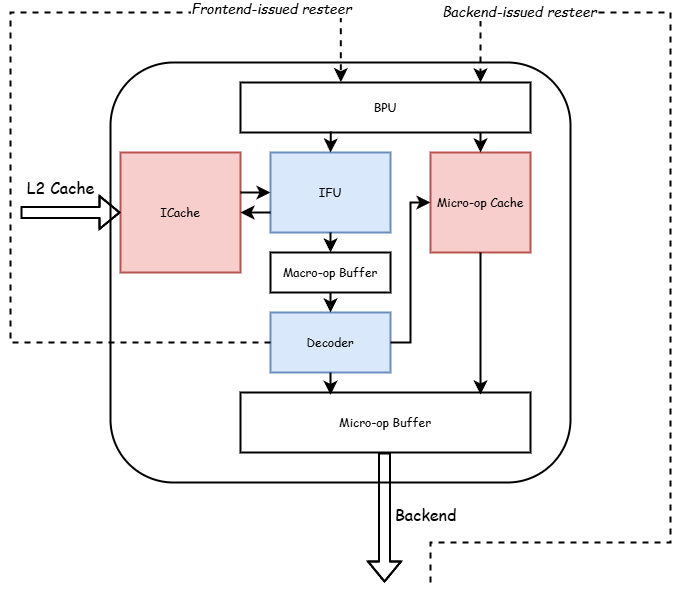
\includegraphics[width=0.6\textwidth]{Figure/decode pipeline.png}
    \end{center}
\end{frame}

\begin{frame}
    \frametitle{Phantom}
    \framesubtitle{Phantom on x86}
    Branch Prediction
    \begin{itemize}
        \item Prediction on instruction type.
        \item Prediction on branch target.
    \end{itemize}
    
    Misprediction Resteer
    \begin{itemize}
        \item Frontend Resteer:
            \begin{itemize}
                \item Mismatch of predicted instruction types.
                \item Incorrect branch prediction address (Direct branch).
            \end{itemize}
            
        \item Backend Resteer:
            \begin{itemize}
                \item Taken/Not-taken conditional branch.
                \item Incorrect branch prediction address (Indirect branch).
            \end{itemize}
    \end{itemize}
\end{frame}

\begin{frame}
    \frametitle{Phantom}
    \framesubtitle{Phantom on x86}
    \begin{minipage}{0.5\textwidth}
        Phantom
        \begin{itemize}
            \item Exploit transient window caused by frontend resteer.
        \end{itemize}
        
        Phantom Workflow
        \begin{itemize}
            \item Train A with direct / indirect branch to C.
            \item Execute B at aliased address to trigger misprediction to C.
            \item Set up observation channel to monitor C's advance in pipeline.
        \end{itemize}
    \end{minipage}
        \hfill
    \begin{minipage}{0.4\textwidth}
        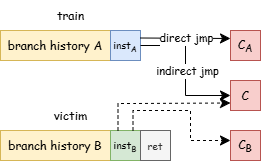
\includegraphics[width=\textwidth]{Figure/trainning overview.png}
    \end{minipage}    
    
\end{frame}

\begin{frame}
    \frametitle{Phantom}
    \framesubtitle{Phantom on x86}
    IF Channel
    \begin{center}
        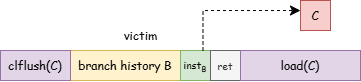
\includegraphics[width=0.45\textwidth]{Figure/IF Channel.png}
    \end{center}
    ID Channel
    \begin{center}
        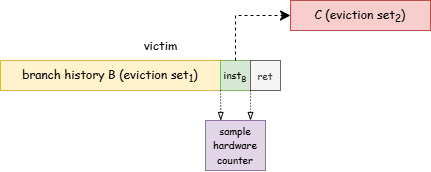
\includegraphics[width=0.5\textwidth]{Figure/ID Channel.png}
    \end{center}
    EX Channel
    \begin{center}
        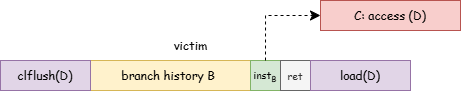
\includegraphics[width=0.5\textwidth]{Figure/EX Channel.png}
    \end{center}
\end{frame}

\begin{frame}[fragile]
    \frametitle{Phantom}
    \framesubtitle{Phantom on x86}
    Example: IF Channel
    \begin{lstlisting}
    for (int j = 0; j < 8; j++)
        train_func();
    memory_barrier //asm volatile("sfence;\nmfence;\nlfence")
    clflush((void*)monitor_addr); 
    memory_barrier
    victim_func();
    delayloop(100000);
    memory_barrier
    uint64_t tim = memaccesstime((void*)monitor_addr);
    \end{lstlisting}
\end{frame}

\begin{frame}[fragile]
    \frametitle{Phantom}
    \framesubtitle{Phantom on x86}
    Hardware Performance Counter used in ID Channel 
    \begin{itemize}
        \item Zen2
            \begin{itemize}
                \item \textit{de\_dis\_uops\_from\_decoder.de\_dis\_uops\_from\_opcache}
                \item \textit{de\_dis\_uops\_from\_decoder.de\_dis\_uops\_from\_both}
            \end{itemize}
        \item Zen3
            \begin{itemize}
                \item \textit{op\_cache\_hit\_miss.op\_cache\_miss}
            \end{itemize}
    \end{itemize}
\end{frame}


\begin{frame}
    \frametitle{Phantom}
    \framesubtitle{Phantom on x86}
    \begin{minipage}{0.5\textwidth}
        
        Trigger misprediction
            \begin{itemize}
                \item Create aliased address:
                    
                    Flip 19th bit and 31st bit on Zen2, 21st bit and 33rd bit on Zen3.
                \item Set up branch history:
                    
                    4$\sim$8 direct jumps separated by 128 bytes.
            \end{itemize}
        
    \end{minipage}
    \hfill
    \begin{minipage}{0.4\textwidth}
        \begin{center}
            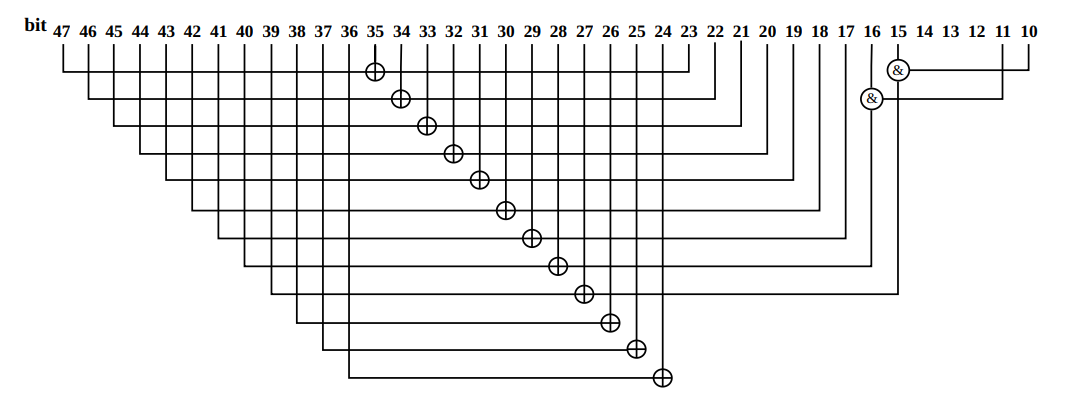
\includegraphics[width=\textwidth]{Figure/Zen2 tag.png}
            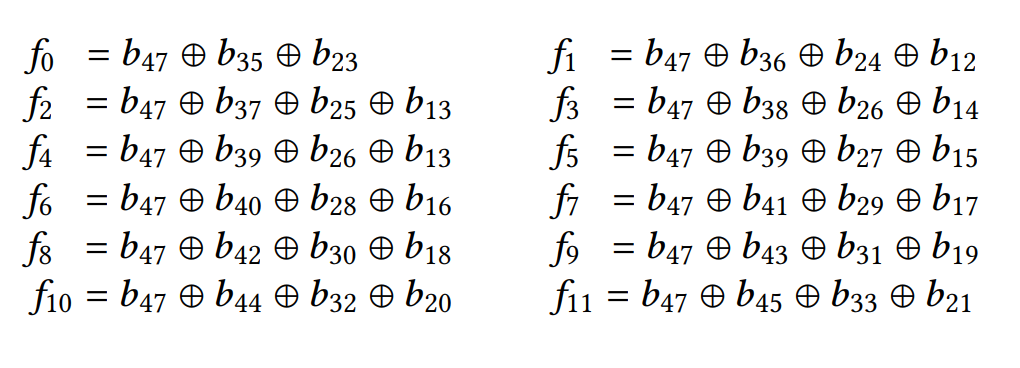
\includegraphics[width=\textwidth]{Figure/Zen3 tag.png}
        \end{center}
    \end{minipage}
\end{frame}

\begin{frame}
    \frametitle{Phantom}
    \framesubtitle{Phantom on XiangShan}
    Nanhu Frontend
    \begin{center}
        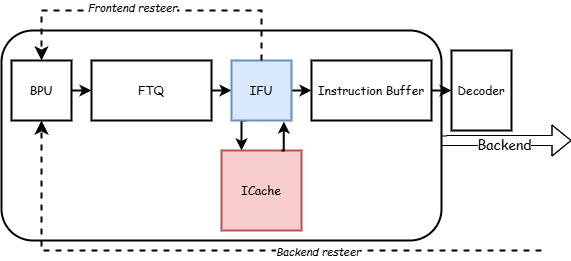
\includegraphics[width=0.7\textwidth]{Figure/xs-frontend.png}
    \end{center}
    Main Different:
    \begin{itemize}
        \item No $\mu$op cache.
        \item Integrated Instruction Fetch and Prediction Check.
    \end{itemize}
\end{frame}

\begin{frame}
    \frametitle{Phantom}
    \framesubtitle{Phantom on XiangShan}
    Observation Channel
    \begin{itemize}
        \item IFU
        \textit{frontend\_icache\_miss\_cnt}, \textit{frontend\_flush}
        \item Decoder
        \textit{ctrlblock\_decoder\_utilization}
    \end{itemize}
    Trigger misprediction
    \begin{itemize}
        \item Create aliased address:

            Using same lower 29 bits
        \item Set up branch history:
            
           32 direct jumps separated by 64 bytes.
    \end{itemize}
    
\end{frame}


\begin{frame}
    \frametitle{Downfall}
    \framesubtitle{Gather Data Sampling}
    Execution of gather instruction\cite{downfall}
    \begin{center}
        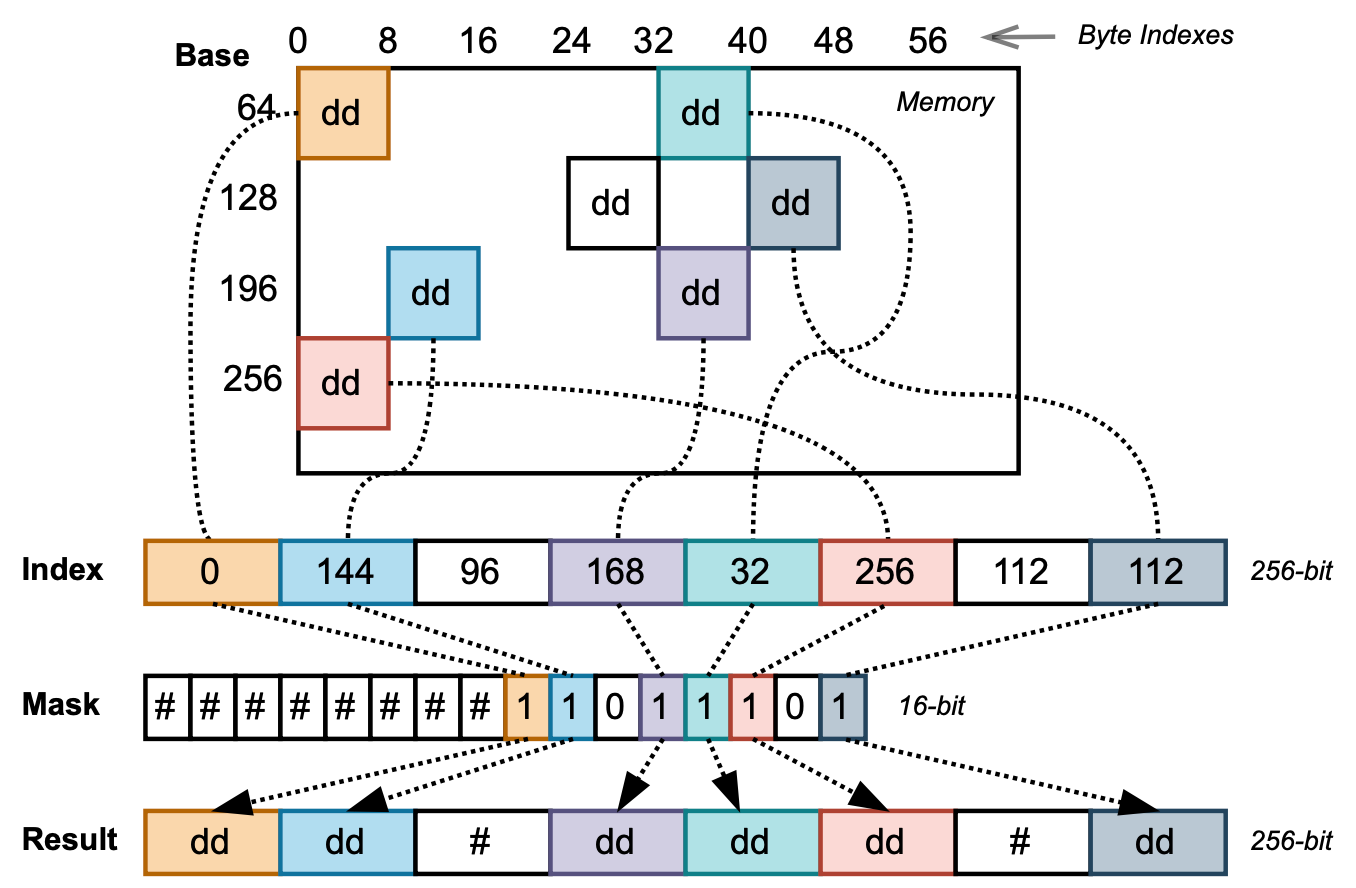
\includegraphics[width=0.7\textwidth]{Figure/gather.png}
    \end{center}
\end{frame}

\begin{frame}
    \frametitle{Downfall}
    \framesubtitle{Gather Data Sampling}
    Microarchitectural data sampling exploits
    \begin{itemize}[<+->]
        \item buffers inside microarchitectural components like load buffer, store-commit buffer
        \item x86 has hyperthreading tech, allowing two threads run on the same core sharing the same resource $\rightarrow$ potential data stealing
        \item hard to conduct, since data in buffer vanished quickly
        \item \texttt{gather} magnifies the attack by filling up the buffer with vector load
        \item then encoding
    \end{itemize}
\end{frame}

\begin{frame}
    \frametitle{Downfall}
    \framesubtitle{Kunminghu Architecture}
    \begin{center}
        \includesvg[width=0.6\textwidth]{Figure/xs-arch-kunminghu.svg}
    \end{center}
\end{frame}

\begin{frame}
    \frametitle{Downfall}
    \framesubtitle{RISC-V Vector Extension}
    Similar to Intel's AVX and ARM's SVE
    \begin{itemize}[<+->]
        \item XiangShan adds on 32 128-bit vector registers and 7 vector CSR
        \item setting vtype and vlen before computing vectors
        \item Vector load, indexed (gather): vlxb, vlxbu, vlxh, vlxhu, vlxw, vlxwu, vlxd, vflxh, vflxw, vflxd
        \item XiangShan reuse the Load-Store Unit in execution of vector instruction $\rightarrow$ GDS attack
    \end{itemize}
\end{frame}

\begin{frame}[fragile]
    \frametitle{Downfall}
    \framesubtitle{Exploiting RVV Instruction}
    Downfall with RVV
    \begin{lstlisting}
    fence.i
    // increase the transient window
    vsetvli t0, %[vl], e64, m1 
    // Set vector length and element width to 64 bits
    vmv.v.x v0, %[mask]
    // Move mask to vector register v0
    vle32.v v2, (%[indices])
    // Load indices into vector register v2
    vluxei64.v v1, (%[src]), v2, v0.t
    // Load 64-bit elements using indices and mask
    vse64.v v1, (%[dst]) Store loaded elements to dst

    encode_secret
    flush_and_reload
    \end{lstlisting}
\end{frame}

\begin{frame}
    \frametitle{Experiment}
    \begin{table}[!htbp]
	\centering
	\begin{tabular}[c]{lll}
		\toprule
        CPU & Generation & Memory \\
		\midrule
        Xeon(R) Silver 4210 & Cascade Lake & DDR4 128GB \\
        AMD R9-3900X  & Zen2 & DDR3 32GB\\
        XiangShan & Nanhu (FPGA) & DDR3 16GB \\
        XiangShan & Kunminghu (Verilator \& GEM5) & DDR3 8GB \\
		\bottomrule 
	\end{tabular}
    \caption{Tested machines}
\end{table}

\onslide<2>{
    \begin{table}[!htbp]
	\centering
	\begin{tabular}[c]{llll}
		\toprule
        CPU & Spectre & Phantom & Downfall \\
		\midrule
        Xeon(R) Silver 4210   & \checkmark &            & \checkmark \\
        AMD R9-3900X             &            & \checkmark &  \\
        XiangShan (Nanhu)     & \checkmark & Ongoing & No RVV \\
        XiangShan (Kunminghu) &  &  & Ongoing \\
		\bottomrule 
	\end{tabular}
    \caption{Result}
    \end{table}
}
\end{frame}

\begin{frame}
    \frametitle{Future Work}
    We plan to work on..
    \begin{itemize}
        \item continue to implement the remaining attacks on XiangShan
        \item propose defense techniques and implement on XiangShan
        \item explore more attack surfaces on XiangShan and RISC-V
    \end{itemize}
\end{frame}

\begin{frame}
    \frametitle{Conclusion}
    \begin{itemize}
        \item Validated side-channel attacks on x86\newline
        Spectre v1, Phantom, and Downfall
        \item Theoretically proved that side-channel attacks on XiangShan and partly implement them\newline
        trying to overcome the inconvenience in the ecosystem
        \item Continue implementing attacks on RISC-V
        \item Plan to mitigate the side-channels on RISC-V
    \end{itemize}
\end{frame}

\begin{frame}[allowframebreaks]{References}
\tiny
\printbibliography
\end{frame}
\end{document}
